\chapter{New Material}
\chapterauthor{Jeff Yoshimi}

% See comments at New_Material_1.tex

\section{New Material for Hebbian Update}

We've seen how the Hebb rule works for scalar values. Nice and easy: if they fire together, wire together; source times target activations.  The situation is the same when we vectorize the rule, but now we have activation vectors $\mathbf{a}_{\text{in}}$ and $\mathbf{a}_{\text{out}}$, and we have to find a vector operations that ``lines up'' the right components of the two vectors so that we strengthen the right ones.  Here is a preview: multiply the output activation column vector times the input row vector (the input transposed, since we assume columns to start), and out pops what we're looking for. 

So, as usual in the vector world, things end up feeling kind of backwards, we multiply output times input rather than the other way around, and there is this mysterious transpose thrown in.  But if we go back to the ``bridge'' panel of the figure above, it ends up making sense. Figure \ref{vectorizedHebb} shows the idea. I like to start in the center panel, and then (to link to the linear algebra) think of the mentally moving the output vector to the left and moving the input vector to the top. Then we have a kind of outer product representation, and all the products kind of line up in the right way. 


\begin{figure}[h]
\centering
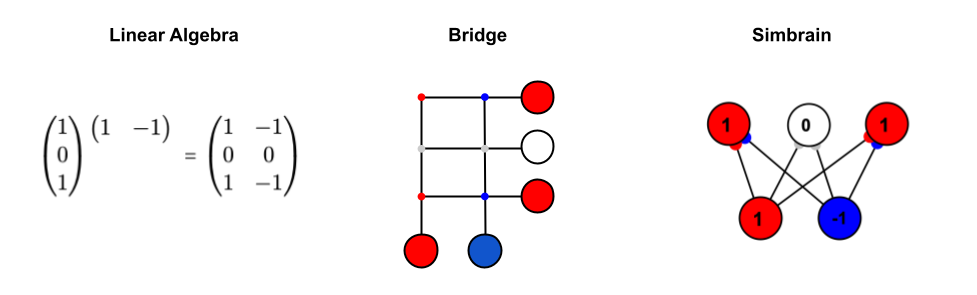
\includegraphics[width=0.9\textwidth]{images/vectorizedHebb.png}
\caption[Jeff Yoshimi.]{Using our visual conventions to conceptualized the vectorized Hebb rule,}
\label{vectorizedHebb}
\end{figure}

 As a slogan: output column times input row gives you a weight matrix.

As a sanity check in the example, check the shapes. We ahve a $3 \times 1$ output vector times a $1 \times 2$ row vectors, which gives us a weight matrix (or weight matrix delta) in the correct shape: $3 \times 2$. This is sometimes called an outer product.
So the vectorized Hebb rule is: 

% Be consistent about symbol for learning rate

Ok, so here is the vectorized Hebb rule:

\begin{eqnarray*}
\Delta \mathbf{w}  = \epsilon \mathbf{a}_{\text{out}} \mathbf{a}_{\text{in}} ^T
\end{eqnarray*}
Remember, by default all vectors in bold face are column vectors.  So this is a column vector (the output activation  $\mathbf{a}_{\text{out}}$) times a row vector (the input activations) which produces a matrix in the same shape as the weight matrix. Again, it feels backwards: we go from target to source (rather than source to target), just to get things in the right format.

The Hebb rule can also be vectorized. Suppose we have an input vector $\mathbf{x} = (1, -1)$, and an output vector $\mathbf{y} = (1,0,1)$. Remember, on an output-input representation, the weight matrix connecting them is $3 \times 2$. So our weight updates, assuming a learning rate of 1, correspond to all the connections between the entries in these two vectors. 

Here is an example
%\[
%\Delta \mathbf{w}  = 
%\begin{pmatrix} 1 \\ 0 \\ 1 \end{pmatrix}
%\begin{pmatrix} 1 & -1 \end{pmatrix}
%=
%\begin{pmatrix}
%    1 & -1 \\
%    0 & 0 \\
%    1 & -1
%\end{pmatrix}
%\]


Our values are
\begin{equation*}
\epsilon = 1 \; \; \; \; \\
\mathbf{a}_{\text{in}} = \begin{bmatrix} 1 \\ -1 \end{bmatrix} \\ 
\; \; \mathbf{a}_{\text{out}} = \begin{bmatrix} 1 \\ 0 \\ 1 \end{bmatrix}
\end{equation*}

Then the equation is (Once they are lined up like this it's kind of easy to ``see'' what is happening, especially in the bridge picture; all the cross points multiply)

\begin{align*}
\Delta \mathbf{w}  = 1
\begin{bmatrix} 1 \\ 0 \\ 1 \end{bmatrix} 
\begin{bmatrix} -1 & 1 \end{bmatrix} 
= \begin{bmatrix} 1 \cdot -1 & 1 \cdot 1 \\ 0 \cdot -1 & 0 \cdot 1 \\ 1 \cdot -1 & 1 \cdot 1 \end{bmatrix} 
= \begin{bmatrix} -1 & 1 \\ 0 & 0 \\  -1 & 1  \end{bmatrix}
\end{align*}

So we get

\begin{align*}
\mathbf{w} + \Delta \mathbf{w}  =
\begin{bmatrix} 0 & 0 \\ 0 & 0 \\  0  & 0  \end{bmatrix} +
\begin{bmatrix} -1 & 1 \\ 0 & 0 \\  -1 & 1  \end{bmatrix} =
\begin{bmatrix} -1 & 1 \\ 0 & 0 \\  -1 & 1  \end{bmatrix}
\end{align*}

Iterate again (assuming we are clamping the nodes; if we weren't the output activations would also be changing) and get


\begin{align*}
\mathbf{w} + \Delta \mathbf{w}  =
\begin{bmatrix} -1 & 1 \\ 0 & 0 \\  -1 & 1  \end{bmatrix} +
\begin{bmatrix} -1 & 1 \\ 0 & 0 \\  -1 & 1  \end{bmatrix} =
\begin{bmatrix} -2 & 2 \\ 0 & 0 \\  -2 & 2  \end{bmatrix}
\end{align*}

 Keep iterating and the entries at the top and bottom right will explode to positive infinity, and the top and bottom right will explode to negative infinity. This can be seen graphically in the Simbrain neuron array representation.
 
Try some other numbers and verify that as you repeatedly iterate, error will get smaller.

% TODO: Redraw a new pic just for vectorized hebb with all the right colors and values


\section{Backprop}

So this is the same thing, we take row error and use it the same way at the output row, but have to do a bit more work to get the hidden layers.

In terms of applications to cognitive science, there is this old work from Zipser that can be used to justify it!

\section{Batches}

This can all be done in pure linear algebra. But it can also be done in a looping way, that might be easier to learn. Then again good to be good with the weight multiplications. Not sure which is best. Maybe both?
